\part{Lógica Temporal Lineal}
\section{Estructuras de Kripke}
\begin{definicion}{Estructura de Kripke}
Una \textbf{estructura de Kripke} es un par $(W,R)$ tal que:
\begin{itemize}
\item $W$ es un conjunto de nodos,
\item $R$ es una relación binaria sobre $W$ ($R\subseteq W\times W$).
\end{itemize}

O sea que es \textbf{es un grafo}. 
\end{definicion}

\begin{definicion}{Función de evaluación}
Una \textbf{función de evaluación} $v:Pr\times W \to \{T,F\}$ asigna a cada proposición un valor de verdad en cada estado del posible.
\end{definicion}

Las estructuras de Kripke, junto con una función de evaluación nos permite representar un programa en base a las propiedades que se deben cumplir en cada uno de sus estados. Cada estado es un nodo y se une con flechas a todos los estados a los que puede pasar el programa desde ese estado. La función de evaluación, nos indica que propocisiones son validad en cada momento de la ejecución.

\paragraph{Ejemplo de Modelo con Krikpe}
\begin{center}
    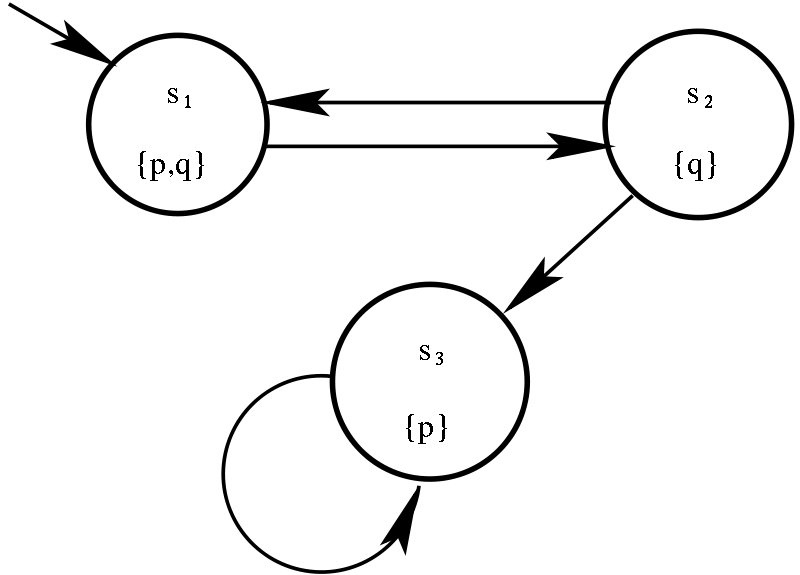
\includegraphics[scale=0.3]{imagenes/kripke.png}
\end{center}

El kripke representa un programa de tres estados $W=\{s_1,s_2,s_3\}$ en el que pueden valer dos proposiciones $p$ y $q$. En cada estados, marcamos cuales de ellas vale entre llaves. Osea que en $s_1$ valen las dos, en $s_2$ vales solo $q$ y en $s_3$ solo $p$.

\begin{definicion}{Traza}
Una traza de una estructura de Kripke son una secuencia infinita de estados $\sigma = \{\sigma_0,\sigma_1,\dots\}$ que representa la ejecución de un programa. $\sigma_i$ representa el estado al que llegó el programa en el $i$-ésimo paso.
\end{definicion}

\newpage
Sean $\psi$ una fórmula de LTL:
\section{Lógica temporal lineal (LTL)}
\begin{itemize}
\item Variables proposicionales: $p,~q,~r,\dots$
\item Conectivos lógicos clásicos: 
\begin{multicols}{2}
\begin{itemize}
\item Conjunción $(\psi_1 \land \psi_2)$
\item Disyunción $(\psi_1 \lor \psi_2)$
\item Negación $(\lnot \psi)$
\item Implicación $(\psi_1 \implies \psi_2)$
\end{itemize}
\end{multicols}
\item Operadores modales:
\begin{multicols}{2}
\begin{itemize}
\item Siempre ($\square \psi$ ó G$\psi$)
\item Eventualmente ($\Diamond \psi$ ó F$\psi$)
\item En el próximo paso (X$\psi$)
\item Hasta que ($\psi_1$ U $\psi_2$)
\end{itemize}
\end{multicols}
\end{itemize}

Nos va a servir para hablar sobre propiedades de alguna ejecución de un programa, es decir, sobre propiedades de alguna de las trazas de un modelo de Kripke.


\subsection{Semántica}
Dada una estructura de Kripke $(W,R)$, una función de evaluación $v$ y $\sigma$ una traza del Kripke decimos que un estado $w$ satisface la formula $\psi$ si $\psi$ es verdadera en ese estado. Sea $p$ una proposicion de la lógica modal, entonces:
\begin{itemize}
    \item $\sigma[i] \vDash p$ si y solo si $v(p,\sigma[i])$
    \item $\sigma[i] \vDash \lnot\psi$ si y solo si $\sigma[i] \nvDash \psi$
    \item $\sigma[i] \vDash \psi_1\land\psi_2$ si y solo si $\sigma[i] \vDash \psi_1$ y $\sigma[i] \vDash \psi_2$.
    \item $\sigma[i] \vDash \psi_1\lor\psi_2$ si y solo si $\sigma[i] \vDash \psi_1$ o $\sigma[i] \vDash \psi_2$.
    \item $\sigma[i] \vDash \psi_1\implies\psi_2$ si y solo si $\sigma[i] \nvDash \psi_1$ o $\sigma[i] \vDash \psi_2$
    \item $\sigma[i] \vDash \lnot\psi$ si y solo si $\sigma[i] \nvDash \psi$
    \item $\sigma[i] \vDash \text{X}\psi$ si y solo si $\sigma[i+1]\vDash \psi$
    \item $\sigma[i] \vDash \lozenge \psi$ si y solo si $(\exists~j: i \leq j)~\sigma[j] \vDash \psi$
    \item $\sigma[i] \vDash \square \psi$  si y solo si $(\forall~j: i \leq j)~\sigma[j] \vDash \psi$
    \item $\sigma[i] \vDash \psi_1 \text{ U } \psi_2$ si y solo si $(\exists~k: i \leq k) (\sigma[k] \vDash \psi_2 ~\wedge~ ((\forall~j: i \leq j < k)~\sigma[j] \vDash \psi_1))$
\end{itemize}

Decimos que una traza $\sigma$ satisface una formula $\psi$ ($\sigma\vDash\psi$) si y solo si $\sigma[0] \vDash \psi$.


\newpage
\section{Verificación de propiedades}
Decimos que un modelo $M$ (Kripke) satisface un fórmula $\psi$ de LTL si y solo si para toda traza $\sigma$ de $M$, vale $\sigma\vDash\psi$.

\subsection{Autómata de buchi}
\begin{definicion}{Autómata de Büchi}
Son autómatas de estados finitos que reconocen lenguajes de palabras infinitas. Solo aceptan una cadena si pasa infinitas veces por uno o más estados de aceptación.

Los vamos a usar para representar conjuntos de trazas de un sistema que cumplan ciertas propiedades. 
\end{definicion}

\begin{figure}[h]
\centering
	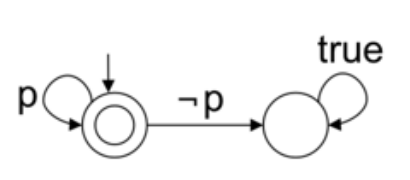
\includegraphics[scale=0.5]{imagenes/buchi-siempre-p}
	\caption{Autómata de buchi para la fórmula $\square p$. Se mantiene en un estado de aceptación mientras valga $p$. En el primer momento que no lo hace, va al segundo estado y se queda ciclando en el mismo (sin importar el valor actual de $p$).}
\end{figure}

\subsection{Método de verificación}
Para comprobar que una fórmula $\psi$ de la lógica temporal es satisfecha por una estructura de Kripke $M$ debemos hacer lo siguiente:
\begin{enumerate}
    \item Convertir la formula $\lnot \psi$  en un autómata de Büchi $A\psi$ \red{(No dijeron como hacer esto, hacerlo por intuición y rogar que este bien)}.
    \item Convertir el Kripke $M$ en un autómata de Büchi $AM$. Todos los estados del autómata generado son de aceptación.
    \item Componer $AM$ con $AP$ (los autómatas de los dos pasos anteriores)
    \item Verificar si el lenguaje que acepta la composición es vació. Debemos buscar un ciclo que contenga un estado de aceptación y sea alcanzable desde el estado inicial.
    \begin{itemize}
    	\item Si el lenguaje es vacío entonces se cumple $\psi$.
    	\item Si no lo es, existe una traza en $M$ que cumple la negación de $\psi$ y funciona como contra ejemplo.
    \end{itemize}
\end{enumerate}
\paragraph{Ejemplo:}
\begin{center}
    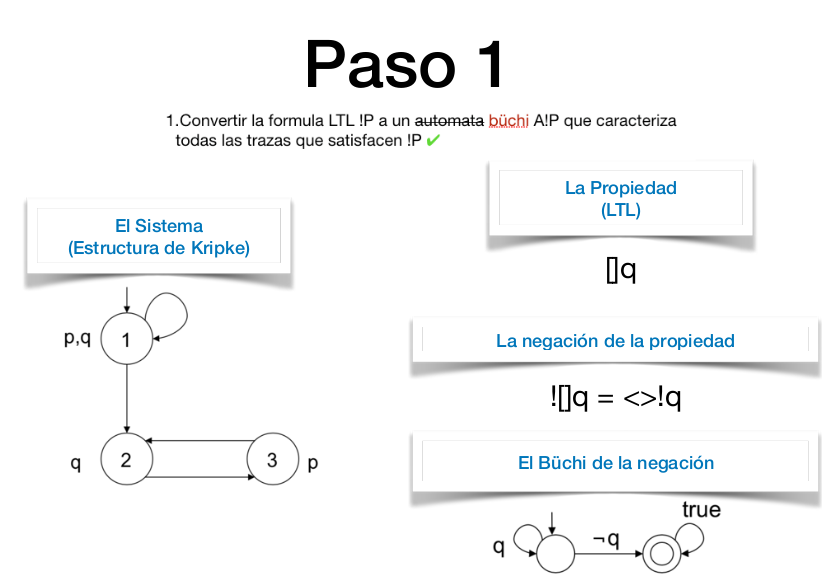
\includegraphics[scale=0.375]{imagenes/paso1.png}
    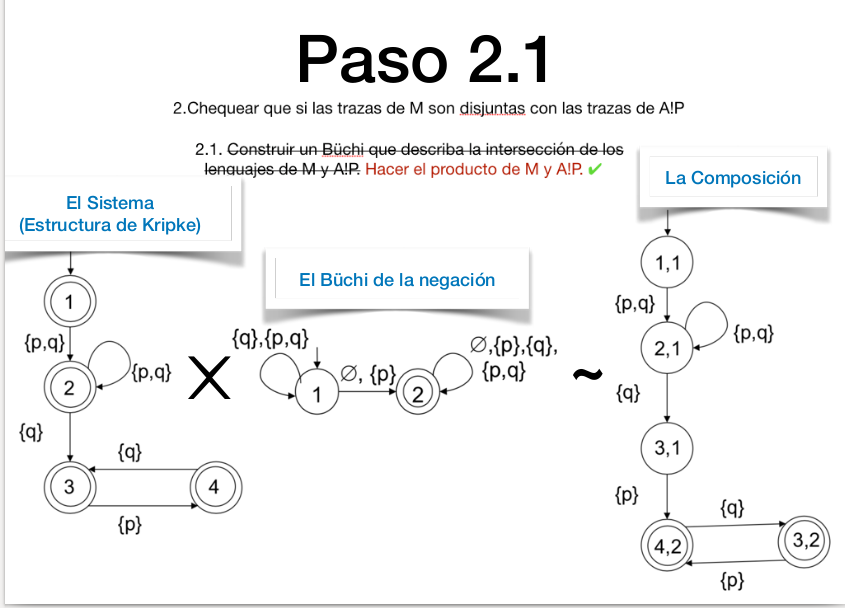
\includegraphics[scale=0.375]{imagenes/paso2.png}
    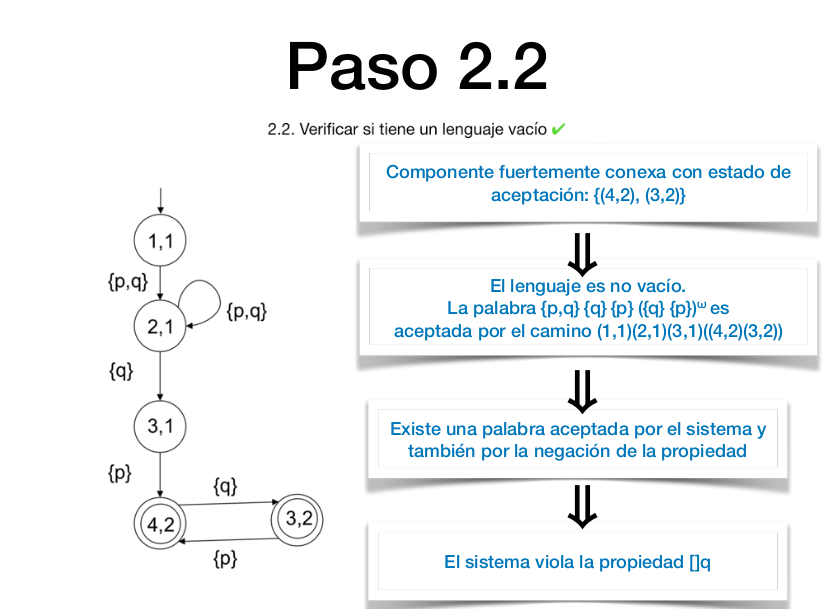
\includegraphics[scale=0.375]{imagenes/paso2-2.png}
\end{center}
